\documentclass[jou]{apa6}

\usepackage[american]{babel}

\usepackage{csquotes}
\usepackage[style=apa,sortcites=true,sorting=nyt,backend=biber]{biblatex}
\DeclareLanguageMapping{american}{american-apa}
\addbibresource{bibliography.bib}


%%%%%%%%%%%%%%%%%%%%%%%%%%%%%%%%%%%%%%%%
%% Discrete Structures
%% The start of RBS stuff
%%%%%%%%%%%%%%%%%%%%%%%%%%%%%%%%%%%%%%%%

% Working internal and external links in PDF
\usepackage{hyperref}
% Extra math symbols in LaTeX
\usepackage{amsmath}
\usepackage{gensymb}
\usepackage{amssymb}
% Enumerations with (a), (b), etc.
\usepackage{enumerate}

\let\OLDitemize\itemize
\renewcommand\itemize{\OLDitemize\addtolength{\itemsep}{-6pt}}

\usepackage{etoolbox}
\makeatletter
\preto{\@verbatim}{\topsep=3pt \partopsep=3pt }
\makeatother

% These sizes redefine APA for A4 paper size
\oddsidemargin 0.0in
\evensidemargin 0.0in
\textwidth 6.27in
\headheight 1.0in
\topmargin -24pt
\headheight 12pt
\headsep 12pt
\textheight 9.19in



\title{Sample Quiz 8}
\author{Discrete Structures, Spring 2020}
\affiliation{RBS}

\leftheader{Discrete Sample Quiz 8}

\abstract{%
}

%\keywords{}

\setlength\parindent{0pt}

\begin{document}

%\thispagestyle{empty}

\twocolumn
\section{Worksheet 11: Graphs}

{\bf Question 1.}\\
{\bf (A)} $K_n$ (the complete graph on $n$ vertices) has $\ldots\ldots$ edges and $\ldots\ldots$ vertices.\\
{\bf (B)} $K_{m,n}$ (the complete bipartite graph on sets of sizes $m,n$) has $\ldots\ldots$ edges and $\ldots\ldots$ vertices.\\
{\bf (C)} $W_n$ (wheel graph on $n$ vertices \textendash{} $n$-gonal pyramid
viewed from above) has $\ldots\ldots$ edges and $\ldots\ldots$ vertices.\\
{\bf (D)} $Q_n$ ($n$-dimensional cube) has $\ldots\ldots$ edges and $\ldots\ldots$ vertices.

\vspace{10pt}
{\bf Question 2 (Rosen7e, Ch.10, Q15-Q17).}\\
{\bf (A)} The length of the longest simple circuit in $K_5$ is $\ldots\ldots$.\\
{\bf (B)} The length of the longest simple circuit in $W_{10}$ is $\ldots\ldots$.\\
{\bf (C)} The length of the longest simple circuit in $K_{4,10}$ is $\ldots\ldots$.

{\em Note.} A simple circuit in (Rosen2019) is defined as a circular
sequence of vertices $v_0,v_1,\ldots,v_n=v_0$, 
where each two neighboring vertices are connected by an edge
(and it does not contain any edge more than once).
It can return to the same vertex multiple times.

\vspace{10pt}
{\bf Question 3 (Rosen7e, Ch.10, Q19-Q24).} In each example find 
the dimensions of a matrix; and number of 0s and 1s in it: Find $X,Y,Z,T$.\\
{\bf (A)} The adjacency matrix for $K_{m,n}$ has size (rows times columns)
$X \times Y$; it has $Z$ 0's and $T$ 1's.\\
{\bf (B)} The adjacency matrix for $K_n$  
has size $X \times Y$; it has $Z$ 0's and $T$ 1's.\\
{\bf (C)} The adjacency matrix for $C_n$  
has size $X \times Y$; it has $Z$ 0's and $T$ 1's.\\
{\bf (D)} The adjacency matrix for $Q_4$  
has size $X \times Y$; it has $Z$ 0's and $T$ 1's.\\
{\bf (E)} The incidence matrix for $W_n$ 
has size $X \times Y$; it has $Z$ 0's and $T$ 1's.\\
{\bf (F)} The incidence matrix for $Q_5$ 
has size $X \times Y$; it has $Z$ 0's and $T$ 1's.

{\em Note.} Adjacency matrix is a square matrix of size $|V| \times |V|$, 
but incidence matrix is a rectangular matrix of size $|V| \times |E|$.

\vspace{10pt}
{\bf Question 4 (Rosen7e, Ch.10, Q28-Q31).}\\
{\bf (A)} List all positive integers $n$ such that $K_n$ has an Euler circuit; 
what is its length in terms of $n$?\\
{\bf (B)} List all positive integers $n$ such that $Q_n$ has an Euler circuit.



\vspace{10pt}
{\bf Question 5 (Rosen7e, Ch.10, Q43).}\\
If $G$ is a planar connected graph with $12$ regions and $20$ edges, then $G$ has $\ldots\ldots$ vertices.


\vspace{10pt}
{\bf Question 6 (Rosen7e, Ch.10, Q44).}\\
If $G$ is a planar connected graph with $20$ vertices, each of degree $3$, then $G$ has $\ldots\ldots$ regions.

\vspace{10pt}
{\bf Question 7 (Rosen7e, Ch.10, Q45).}\\
If a regular graph $G$ has $10$ vertices and $45$ edges, then each vertex of $G$ has degree $\ldots\ldots$.

{\em Note.} A {\em regular graph} is a graph where all vertices have the same degree.



\vspace{10pt}
{\bf Question 8 (Rosen7e, Ch.10, Q59-Q82).}\\
{\bf (A)} A simple graph with $6$ vertices, whose degrees are $2,2,2,3,4,4$.\\
{\bf (B)} A simple graph with $8$ vertices, whose degrees are $0,1,2,3,4,5,6,7$.\\
{\bf (C)} A simple graph with degrees $1,2,2,3$.\\
{\bf (D)} A simple graph with degrees $2,3,4,4,4$.\\
{\bf (E)} A simple graph with degrees $1,1,2,4$.\\
{\bf (F)} A simple digraph with indegrees $0,1,2$ and outdegrees $0,1,2$.\\
{\bf (G)} A simple digraph with indegrees $1,1,1$ and outdegrees $1,1,1$.\\
{\bf (H)} A simple digraph with indegrees $0,1,2,2$ and outdegrees $0,1,1,3$.\\
{\bf (I)} A simple digraph with indegrees $0,1,2,4,5$ and outdegrees $0,3,3,3,3$.\\
{\bf (J)} A simple digraph with indegrees $0,1,1,2$ and outdegrees $0,1,1,1$.\\
{\bf (K)} A simple digraph with indegrees: $0,1,2,2,3,4$ and outdegrees: $1,1,2,2,3,4$.\\
{\bf (L)} A simple graph with $6$ vertices and $16$ edges.\\
{\bf (M)} A connected simple planar graph with $5$ regions and $8$ vertices, each of degree $3$.\\
{\bf (N)} A graph with $4$ vertices that is not planar.\\
{\bf (O)} A planar graph with $10$ vertices.\\
{\bf (P)} A planar graph with $8$ vertices, $12$ edges, and $6$ regions.\\
{\bf (Q)} A planar graph with $7$ vertices, $9$ edges, and $5$ regions.



\vspace{10pt}
{\bf Question 9 (Rosen7e, Ch.10, Q108).}\\
Use Dijkstra’s Algorithm to find the shortest path length between 
the vertices a and z in these weighted graphs.

{\bf (A)}
\begin{figure}[!htb]
\center{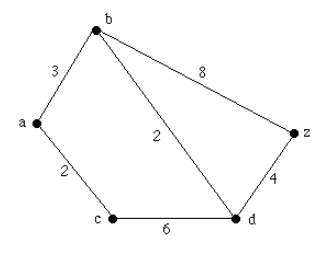
\includegraphics[width=2in]{quiz-sample-11/dijkstra-graph1.png}}
\caption{\label{fig:dijkstra-graph1} Weighted graph 1.}
\end{figure}

\newpage
{\bf (B)}
\begin{figure}[!htb]
\center{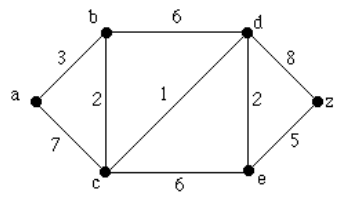
\includegraphics[width=2in]{quiz-sample-11/dijkstra-graph2.png}}
\caption{\label{fig:dijkstra-graph2} Weighted graph 2.}
\end{figure}


\vspace{10pt}
{\bf Question 10 (Rosen7e, Ch.10, Q113).}\\
The picture at the right shows the floor plan of
an office. Show that it is impossible to plan a walk that passes through
each doorway exactly once, starting and ending at $A$.
\begin{figure}[!htb]
\center{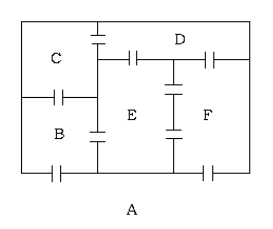
\includegraphics[width=2in]{quiz-sample-11/floor-plan-graph.png}}
\caption{\label{fig:floor-plan-graph} Floor plan.}
\end{figure}


\vspace{10pt}
{\bf Hall's Marriage Theorem (Rosen2019, p.772)}\\
The bipartite graph $G=(V,E)$ with partition 
of vertices into 2 disjoint sets $V = X \cup Y$ 
has a {\em maximum matching} that saturates $X$
iff for all $A \subseteq X$ we have
$|X| \leq |N(X)|$. 

{\em Note.} A {\em matching} in a graph is a set of of edges
such that no two edges share a common endpoint. 
A {\em maximum matching} is matching containing the greatest
number of edges. And a matching {\em saturates} a set $X$, 
if each vertex $v \in X$ belongs to some matching edge.

\vspace{10pt}
{\bf Question 11 (K\"{o}nig’s Marriage Theorem)}\\
Prove that if all the vertices of a bipartite graph
have the same degree, then it has a perfect matching.\\
(Quines2017, p.11); \url{https://cjquines.com/files/halls.pdf}

{\em Note.} A matching is {\em perfect}, if it saturates all vertices
(every vertex has a pair).

\vspace{10pt}
{\bf Question 12}\\
We have a regular deck of $52$ playing cards, with exactly $4$ cards of each of the
13 ranks. The cards have been randomly dealt into 13 piles, each with 4 cards in
it. Prove that there is a way to take a card from each pile so that after we take
a card from every pile, we have exactly a card of every rank.\\
(Quines2017, p.11).


\newpage
\subsection{Answers}

\vspace{10pt}
{\bf Question 1.} Answer:\\

{\bf (A)} $K_n$ has $\frac{n(n-1)}{2}$ edges and $n$ vertices.\\
{\bf (B)} $K_{m,n}$ has $m \cdot n$ edges and $m+n$ vertices.\\
{\bf (C)} $W_n$ has $2n$ edges and $n+1$ vertices.\\
{\bf (D)} $Q_n$ has $n \cdot 2^{n-1}$ edges and $2^n$ vertices.

The number of edges in $Q_n$ could be first expressed by a recurrent formula
(and then proven by mathematical induction).

\vspace{10pt}
{\bf Question 2.} Answer: TBD\\

\vspace{10pt}
{\bf Question 3.} Answer: TBD\\

\vspace{10pt}
{\bf Question 4.} Answer: TBD\\

\vspace{10pt}
{\bf Question 5.} Answer: TBD\\

\vspace{10pt}
{\bf Question 6.} Answer: TBD\\

\vspace{10pt}
{\bf Question 7.} Answer: TBD\\

\vspace{10pt}
{\bf Question 8.} Answer: TBD\\

\vspace{10pt}
{\bf Question 9.} Answer: TBD\\

\vspace{10pt}
{\bf Question 10.} Answer: TBD\\

\vspace{10pt}
{\bf Question 11.} Answer: TBD\\

\vspace{10pt}
{\bf Question 12.} Answer: TBD\\




\end{document}

